\documentclass[acmsmall,anonymous,nonacm]{acmart}

%% --- preamble ------------------------------------------------------------
\settopmatter{printacmref=false}
\setcopyright{none}
\renewcommand\footnotetextcopyrightpermission[1]{}
\acmJournal{TQC}

\usepackage{amsmath}
\usepackage{tikz}
\usetikzlibrary{positioning,fit,backgrounds,calc,arrows.meta}
\usepackage{pgfplots}
\pgfplotsset{compat=1.16}
\usepackage{algorithm}
\usepackage{algpseudocode}
\usepackage{multirow}

% chain colours reused across figures
\definecolor{chA}{RGB}{214,39,40}
\definecolor{chB}{RGB}{31,119,180}
\definecolor{chC}{RGB}{44,160,44}
\definecolor{chD}{RGB}{255,127,14}

\begin{document}

\title{PathFinder: Negotiated-Congestion Rip-up-and-Reroute for Minor Embedding
on D-Wave Quantum Annealers}

\author{Anonymous Author(s)}
\affiliation{%
  \institution{Anonymous Institution}
  \country{}
}

\begin{abstract}
Minor embedding---mapping a logical problem graph onto the fixed sparse
connectivity of a quantum annealer by representing each logical variable as a
connected \emph{chain} of physical qubits---is the compilation bottleneck for
quantum annealing. The de facto standard, \texttt{minorminer}, is a randomized
rip-up-and-reroute heuristic whose chains are built as unions of independent
shortest paths and whose congestion signal is a memoryless per-pass snapshot;
both choices inflate the \emph{average chain length} (ACL), the metric most
widely taken as the primary proxy for embedded-problem solution quality, and
produce high run-to-run variance. We observe that chain construction is exactly the multi-net global
routing problem solved for thirty years in FPGA/VLSI computer-aided design, and
port its two key ideas to minor embedding: a true Steiner-tree inner step
(the shortest-path heuristic) in place of independent shortest paths, and
\emph{negotiated congestion} (McMurchie--Ebeling) in place of the snapshot
penalty. We package these as PathFinder, an anytime, large-neighbourhood
\emph{improver} that warm-starts from a fast base embedding and then rips up and
reroutes the longest chains through a congestion-priced fabric, accepting a move
only if it lowers the total qubit count and preserves validity---so it never
returns an embedding worse than its base. The algorithmic primitives are classical; the
contribution is their synthesis and application to minor embedding, together
with an empirical evaluation inside the Ember benchmarking framework. On
Erd\H{o}s--R\'enyi, $d$-regular, and Barab\'asi--Albert sources embedded into
clean and broken D-Wave Pegasus and into Zephyr (all four methods reach $100\%$
success on every target), \texttt{pathfinder} never returns a longer-ACL
embedding than \texttt{minorminer} on any of the $35$ instance--topology cells,
and its thorough configuration lowers mean ACL on every cell (by $1$--$11\%$,
mean ${\sim}5\%$) and reduces ACL standard deviation in $30$ of the $35$ (by up
to $77\%$), at the cost of additional wall-clock time. We then optimize the
algorithm---bounded-region routing, a dirty-set incremental schedule, and a
spur-pruning finishing pass---making the production improver $\sim$3$\times$
faster at equal-or-better ACL: single-seed \texttt{pathfinder} runs within
${\sim}1.3\times$ compiled \texttt{minorminer}'s wall-clock while still
shortening mean ACL, and the optimized thorough configuration reaches ${-}5\%$
mean ACL (up to ${-}11\%$) at a fraction of its former cost. Finally, treating
PathFinder's outputs as training data, we ask whether an \emph{amortized} model can
learn to embed: a generative graph variational autoencoder that samples several
candidate hardware layouts and keeps the best matches \texttt{pathfinder-thorough}'s
mean ACL and attains the \emph{lowest} run-to-run ACL variance of any method we
tested---learned or heuristic---on both Pegasus and Zephyr, at full validity.
\end{abstract}

\ccsdesc[500]{Hardware~Quantum computation}
\ccsdesc[300]{Theory of computation~Routing and layout}
\ccsdesc[300]{Mathematics of computing~Graph algorithms}

\keywords{minor embedding, quantum annealing, D-Wave, graph minors, negotiated
congestion routing, Steiner tree, large-neighbourhood search}

\maketitle

%% ========================================================================
\section{Introduction}
\label{sec:intro}

Quantum annealers such as those built by D-Wave solve optimization problems
encoded as Ising/QUBO models whose interaction graph is the user's
\emph{logical} (problem) graph. The hardware, however, exposes only a fixed,
sparse \emph{physical} graph---successive D-Wave generations Chimera,
Pegasus~\cite{boothby2020pegasus}, and Zephyr~\cite{boothby2021zephyr} have qubit
degree $6$, $15$, and $20$ respectively. Running a problem
whose interaction graph is denser than the hardware requires \emph{minor
embedding}: each logical variable is realized by a connected set of physical
qubits, a \emph{chain}, whose qubits are forced into agreement by strong
ferromagnetic couplings so that the chain behaves as one logical
spin~\cite{cai2014minorminer,lucas2014ising}.

\paragraph{The minor-embedding problem.}
Let $H$ be the \emph{source} (problem) graph and $G$ the \emph{target}
(hardware) graph. A minor embedding is a map
$\varphi : V(H) \to 2^{V(G)}$ assigning to each logical vertex $v$ a chain
$\varphi(v)\subseteq V(G)$, subject to three conditions:
\begin{enumerate}
  \item \textbf{Connectivity.} Each $\varphi(v)$ induces a connected subgraph
        of $G$.
  \item \textbf{Disjointness.} The chains are pairwise disjoint:
        $\varphi(u)\cap\varphi(v)=\varnothing$ for $u\neq v$.
  \item \textbf{Edge preservation.} For every edge $(u,v)\in E(H)$ there is at
        least one hardware edge between the chains, i.e.\ some
        $a\in\varphi(u)$, $b\in\varphi(v)$ with $(a,b)\in E(G)$.
\end{enumerate}
The map is total with non-empty chains, so every logical vertex is realized;
Ember's validator (\S\ref{sec:ember}) records this as the \emph{coverage} check.
Figure~\ref{fig:embedding} illustrates the conditions. Feasibility is the
question ``does a minor embedding exist?''; in practice one wants the
\emph{best} embedding, because the dominant cost is qubit usage and chain
fidelity. The standard objective is to minimize the \emph{average chain length}
\begin{equation}
  \mathrm{ACL}(\varphi) \;=\; \frac{1}{|V(H)|}\sum_{v\in V(H)} |\varphi(v)|,
  \label{eq:acl}
\end{equation}
and to keep chain lengths \emph{uniform} (low coefficient of variation): long
and unequal chains require stronger chain couplings, shrink the available
dynamic range for the logical problem, and empirically raise the annealer's
solution error. ACL is therefore the headline quality metric, with total qubit
count, maximum chain length, and chain-length uniformity as close companions.

\begin{figure}[t]
\centering
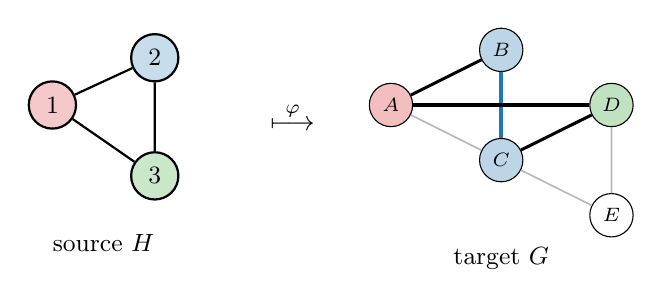
\begin{tikzpicture}[x=1cm,y=1cm,
   lv/.style={circle,draw,thick,minimum size=6mm,inner sep=0pt,font=\small},
   qb/.style={circle,draw,minimum size=5.5mm,inner sep=0pt,font=\scriptsize},
   cpl/.style={gray!55,line width=0.6pt}]
%% ---- source H (triangle 1-2-3) ----
\node[lv,fill=chA!25] (s1) at (0,1.4) {$1$};
\node[lv,fill=chB!25] (s2) at (1.3,2.0) {$2$};
\node[lv,fill=chC!25] (s3) at (1.3,0.5) {$3$};
\draw[thick] (s1)--(s2) (s2)--(s3) (s1)--(s3);
\node at (0.65,-0.35) {\small source $H$};

%% ---- arrow ----
\node at (3.05,1.25) {$\overset{\varphi}{\longmapsto}$};

%% ---- target G with chains ----
\begin{scope}[xshift=4.3cm]
  \node[qb,fill=chA!30] (A) at (0,1.4) {$A$};
  \node[qb,fill=chB!30] (B) at (1.4,2.1) {$B$};
  \node[qb,fill=chB!30] (C) at (1.4,0.7) {$C$};
  \node[qb,fill=chC!30] (D) at (2.8,1.4) {$D$};
  \node[qb] (E) at (2.8,0.0) {$E$};
  % couplers (all light); realized/intra-chain drawn darker
  \draw[cpl] (A)--(C) (C)--(E) (D)--(E);
  \draw[chB,line width=1.4pt] (B)--(C); % intra-chain phi(2)
  \draw[line width=1.1pt] (A)--(B); % H-edge 1-2
  \draw[line width=1.1pt] (C)--(D); % H-edge 2-3
  \draw[line width=1.1pt] (A)--(D); % H-edge 1-3
  \node at (1.4,-0.55) {\small target $G$};
\end{scope}
\end{tikzpicture}
\caption{Minor embedding of the triangle $H$ into a hardware patch $G$.
Vertex $1\!\mapsto\!\varphi(1)=\{A\}$, $2\!\mapsto\!\{B,C\}$,
$3\!\mapsto\!\{D\}$ (matching colours). Chain $\varphi(2)$ is connected through
the bold intra-chain coupler $B\!-\!C$; the three chains are disjoint; each
$H$-edge is realized by a hardware coupler between the corresponding chains
($1\!-\!2$ by $A\!-\!B$, $2\!-\!3$ by $C\!-\!D$, $1\!-\!3$ by $A\!-\!D$). Qubit
$E$ is unused. Here $\mathrm{ACL}=\tfrac{1+2+1}{3}=\tfrac{4}{3}$.}
\label{fig:embedding}
\end{figure}

\paragraph{Contribution.}
This paper makes five contributions. (i) We frame minor-embedding chain
construction as \emph{multi-net global routing} and transfer two ideas from
FPGA/VLSI computer-aided design---a real Steiner-tree inner step and
\emph{negotiated congestion}---to the quantum-annealing setting
(\S\ref{sec:pathfinder}). (ii) We package them as \textbf{PathFinder}, an
anytime, large-neighbourhood \emph{improver} that warm-starts from a fast base
embedding and, by construction, never regresses below it. (iii) We evaluate PathFinder
inside the Ember benchmarking framework (\S\ref{sec:ember}) against
\texttt{minorminer} and \texttt{minorminer}-with-p-norm-layout on clean and
broken Pegasus and on Zephyr (\S\ref{sec:results}), showing it reduces mean
ACL and---the property that most distinguishes it---run-to-run ACL
\emph{variance} in nearly every cell, while all methods retain full success and
validity. (iv) We then \emph{optimize} the algorithm (\S\ref{sec:optimizations}):
a structured pass yields three quality-safe improvements---bounded-region
routing, a dirty-set incremental schedule, and a spur-pruning finishing
pass---that together make the production algorithm $\sim$3$\times$ faster at
equal-or-better ACL, bringing single-seed \texttt{pathfinder} to within
${\sim}1.3\times$ compiled \texttt{minorminer}'s wall-clock. (v) Finally, we ask
whether \emph{learning} helps (\S\ref{sec:learning}): training amortized models on
PathFinder-optimized embeddings, a generative graph variational autoencoder that
samples and selects among candidate hardware layouts matches
\texttt{pathfinder-thorough}'s mean ACL and achieves the lowest run-to-run ACL
variance of any method---learned or heuristic---on both topologies, at full
validity. We are explicit
(\S\ref{sec:novelty}) that the
algorithmic primitives are not new; the novelty is their synthesis and
application to minor embedding (and, for \S\ref{sec:learning}, the empirical finding).

%% ========================================================================
\section{Background and Related Work}
\label{sec:related}

\paragraph{The standard heuristic and its weaknesses.}
\texttt{minorminer} (MM), the Cai--Macready--Roy heuristic~\cite{cai2014minorminer},
is randomized coordinate descent. It fixes a random vertex order and, for each
vertex, rips out its chain and rebuilds it as the union of weighted
shortest-path computations to its already-placed neighbours; qubit contention is
discouraged by a vertex weight $\mathrm{diam}(G)^{k}$ where $k$ is the number of
chains currently using the qubit, recomputed from scratch each pass; it iterates
until the embedding is valid or a patience bound is hit. Three structural
weaknesses follow directly. First, a chain is a \emph{union of independent
shortest paths}---a weak Steiner-tree heuristic that misses shared structure.
Second, the congestion signal is \emph{myopic}: a per-pass snapshot with no
memory of how contested a qubit has been over time. Third, the result is highly
\emph{order- and seed-dependent}. The most recent state-of-the-art
evaluation~\cite{gomez2025eval} documents the consequences on broken Pegasus:
run-to-run ACL can differ by several qubits per chain on the same instance, MM is
beaten by deterministic clique embedding once the source's average degree
exceeds the hardware degree, and MM routinely hits a $\sim$1000\,s cutoff on
large dense instances. The MM paper itself names ``better initial placement of
vertex-models'' as the key open problem.

\paragraph{Deterministic templates.}
For sufficiently structured inputs, embeddings can be read off a template.
Clique (``busclique'') embedding generates complete-graph minors in Chimera and
Pegasus connectivity directly~\cite{boothby2016clique}; complete-bipartite
templates~\cite{sinno2025bipartite} and the 4-clique network on a contracted
hardware graph~\cite{pelofske2024fourclique} extend the idea. These are fast and
uniform but over-provision qubits on graphs that are not near-complete.

\paragraph{Layout- and spring-seeded heuristics.}
A complementary line attacks MM's initial-placement weakness by first laying out
the source graph in a low-dimensional space and placing variables near the
geometrically closest qubits: layout-aware embedding~\cite{pinilla2019layout},
the spring/clique-seeded methods of Zbinden et al.~\cite{zbinden2020embedding},
and Ocean's ``Layout Embedding'', which seeds MM with a $p$-norm layout. We use
the latter as a baseline.

\paragraph{Exact methods.}
Integer-programming formulations with Benders
decomposition~\cite{bernal2020ip} and algebraic-geometry/Gr\"obner-basis
compilers~\cite{dridi2018algebraic} solve minor embedding optimally but do not
scale past tens of vertices.

\paragraph{Metaheuristics and learned policies.}
Path/super-vertex simulated annealing (PSSA)~\cite{sugie2018pssa} and
graph-theoretic OCT/virtual-hardware methods~\cite{goodrich2018oct} apply local
search; more recently, GNN-RL (CHARME~\cite{ngo2024charme}) and PPO
policies~\cite{nembrini2025ppo} learn chain-construction heuristics.

\paragraph{Routing and optimal transport.}
Two threads inform our approach. Negotiated-congestion routing
(PathFinder)~\cite{mcmurchie1995pathfinder} from FPGA CAD treats each net as a
resource consumer that negotiates for congested wires over iterations; and
Gromov--Wasserstein optimal transport~\cite{xu2019gwl,vincentcuaz2022srgw}
matches graphs by their intra-graph distances, suggesting a global, continuous
view of the assignment. Our method develops the first thread; the second is
promising future work (\S\ref{sec:limitations}).

%% ========================================================================
\section{The Preliminary PathFinder Algorithm}
\label{sec:pathfinder}

This section presents PathFinder as first designed; \S\ref{sec:results} reports
its results. A subsequent optimization pass (\S\ref{sec:optimizations}) makes the
production algorithm $\sim$3$\times$ faster at equal-or-better quality without
changing the ideas below, so we keep this preliminary description intact and
report the optimized numbers separately.

\subsection{Minor embedding as multi-net routing}
A chain $\varphi(v)$ that must be connected and adjacent to each neighbour's
chain is exactly a \emph{Steiner tree} (a routing ``net'') whose terminals are
the qubits bordering the neighbour chains, and the disjointness requirement is
exactly the rule that two nets may not share a routing resource. Minor embedding
is therefore a multi-net global routing problem on the graph $G$, and the
mature machinery of FPGA/VLSI routing applies. We import its two central ideas.

\subsection{A real Steiner inner step}
\label{sec:steiner}
Rather than build a chain as a union of independent shortest paths to a single
root (MM), we grow one tree with the classical \emph{shortest-path heuristic}
(SPH)~\cite{takahashi1980sph,mehlhorn1988steiner}: starting from a root, each
neighbour terminal is connected to the \emph{nearest node of the current tree},
so later connections reuse earlier structure. Figure~\ref{fig:steiner}
contrasts the two: when neighbours cluster, SPH shares a trunk and produces a
strictly shorter chain.

\begin{figure}[t]
\centering
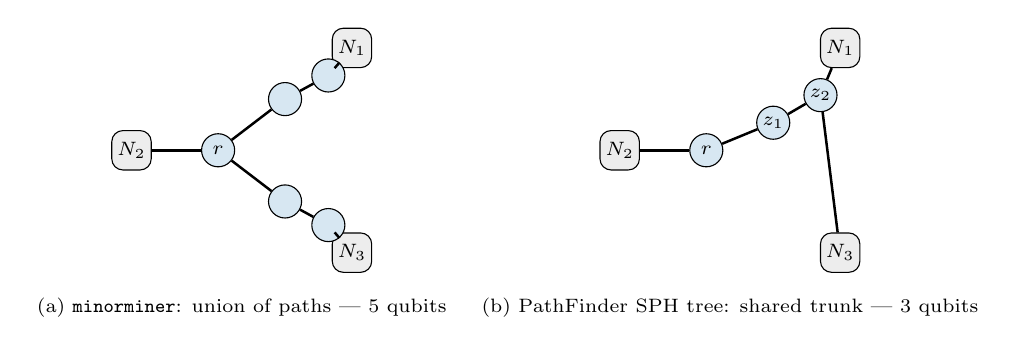
\begin{tikzpicture}[x=1cm,y=1cm,font=\scriptsize,
   q/.style={circle,draw,fill=chB!18,minimum size=4.2mm,inner sep=0pt},
   nb/.style={rounded corners,draw,fill=gray!14,minimum height=5mm,inner sep=2pt},
   e/.style={line width=0.9pt}]
%% ---- panel (a): MM union of shortest paths ----
\begin{scope}
  \node[nb] (N2a) at (-1.1,0) {$N_2$};
  \node[nb] (N1a) at (1.7,1.3) {$N_1$};
  \node[nb] (N3a) at (1.7,-1.3) {$N_3$};
  \node[q] (r) at (0,0) {$r$};
  \node[q] (x1) at (0.85,0.65) {};
  \node[q] (x2) at (1.4,0.95) {};   % path to N1
  \node[q] (y1) at (0.85,-0.65) {};
  \node[q] (y2) at (1.4,-0.95) {};  % path to N3
  \draw[e] (r)--(N2a);
  \draw[e] (r)--(x1)--(x2)--(N1a);
  \draw[e] (r)--(y1)--(y2)--(N3a);
  \node at (0.3,-2.0) {(a) \texttt{minorminer}: union of paths --- $5$ qubits};
\end{scope}
%% ---- panel (b): SPH shared tree ----
\begin{scope}[xshift=6.2cm]
  \node[nb] (N2b) at (-1.1,0) {$N_2$};
  \node[nb] (N1b) at (1.7,1.3) {$N_1$};
  \node[nb] (N3b) at (1.7,-1.3) {$N_3$};
  \node[q] (R) at (0,0) {$r$};
  \node[q] (z1) at (0.85,0.35) {$z_1$};
  \node[q] (z2) at (1.45,0.7) {$z_2$};   % trunk reaching N1
  \draw[e] (R)--(N2b);
  \draw[e] (R)--(z1)--(z2)--(N1b);
  \draw[e] (z2)--(N3b);             % N3 attaches to nearest tree node z2
  \node at (0.3,-2.0) {(b) PathFinder SPH tree: shared trunk --- $3$ qubits};
\end{scope}
\end{tikzpicture}
\caption{Inner step contrast for a chain that must reach three neighbour chains
$N_1,N_2,N_3$. (a) MM routes an independent shortest path to each, duplicating
qubits when $N_1$ and $N_3$ are near each other. (b) The shortest-path-heuristic
Steiner tree attaches $N_3$ to the nearest existing tree node ($z_2$), reusing
the trunk built for $N_1$, yielding a shorter chain.}
\label{fig:steiner}
\end{figure}

\subsection{Negotiated congestion}
\label{sec:negotiation}
We replace MM's snapshot penalty with the negotiated-congestion cost of
McMurchie and Ebeling~\cite{mcmurchie1995pathfinder}. Routing prices each qubit
$q$ at
\begin{equation}
  \mathrm{cost}(q) \;=\; \bigl(1 + h_q\bigr)\,\bigl(1 + \lambda \cdot o_q\bigr),
  \label{eq:cost}
\end{equation}
where $o_q$ is the number of \emph{other} chains currently occupying $q$
(occupancy), $\lambda$ is the present-congestion factor, and $h_q$ is a
\emph{history} term that \emph{accumulates} by a fixed increment every iteration
in which $q$ is over-subscribed. The present term makes a qubit more expensive as
nets pile onto it within a pass; the history term gives the price a memory, so a
persistently contested qubit becomes permanently expensive and the chains that
can most cheaply route around it eventually yield. This is a Lagrangian view of
the disjointness constraint; in FPGA routing it is known to drive the search
toward a legal, low-congestion state, and we observe the same behaviour
here---behaviour MM's memoryless snapshot cannot sustain. A
node-weighted Dijkstra over Eq.~\eqref{eq:cost} supplies the shortest-path
computations the SPH step needs.

\subsection{A warm-started large-neighbourhood improver}
\label{sec:improver}
A from-scratch router that places every chain from scattered single-qubit seeds
is throttled by exactly the open problem MM names---\emph{initial placement}.
Without co-locating adjacent variables, dense-graph chains balloon and the search
often fails to legalize at all. The standalone \texttt{pathfinder-cold} variant
(a cold start followed by the same improver) bears this out: on the nine
clean-Pegasus Erd\H{o}s--R\'enyi instances of our grid
($n\in\{20,30,40\}$, $d\in\{0.3,0.5,0.7\}$) it legalizes only four---the smaller
and sparser ones, at ACL $2.5$--$3.8$---and fails on the five larger, denser ones,
whereas
\texttt{minorminer} embeds all nine
(reproduced by \texttt{docs/paper/data/coldstart\_probe.py}).
PathFinder therefore runs as an \emph{improver}. It warm-starts from a fast base
embedding (MM by default; any registered algorithm works), then performs
\emph{large-neighbourhood} rip-up-and-reroute---the neighbourhood being a long
chain together with the cascade of chains its rerouting displaces. It takes the
longest chain and lets it re-route along the cheapest tree under
Eq.~\eqref{eq:cost}---which may cross occupied territory and create temporary
overlaps---then re-routes every chain it displaced through free space. A move is
committed only if it lowers the embedding's total qubit count (equivalently, its
ACL) and leaves it valid; otherwise the prior state is restored
(Algorithms~\ref{alg:driver}--\ref{alg:move}). Because PathFinder keeps the best
valid embedding it has seen, it \textbf{never returns an embedding worse than its
base}, and it spends its entire time budget reducing ACL---an anytime guarantee
MM's one-shot, patience-bounded run lacks. The \texttt{thorough} configuration
additionally runs four seeded restarts and keeps the best, trading wall-clock for
lower ACL and variance. When no valid base is available, a fallback builds the
initial embedding from scratch in breadth-first vertex order under the same
negotiated cost; uncompetitive on its own, it exists only to guarantee an output.

\begin{algorithm}[t]
\caption{PathFinder (driver)}
\label{alg:driver}
\begin{algorithmic}[1]
\Require source $H$, target $G$, base embedder $\mathcal{B}$
\State $\Phi \gets \mathcal{B}(H,G)$ \Comment{warm start}
\If{$\Phi$ invalid} $\Phi \gets \textsc{ColdStart}(H,G)$ \Comment{BFS-ordered negotiated fallback}
\EndIf
\If{$\Phi$ invalid} \Return failure \EndIf
\State $\Phi^\star \gets \Phi$ \Comment{best valid so far}
\Repeat
  \ForAll{$v \in V(H)$ in decreasing chain length}
     \State $\Phi \gets \textsc{TryShorten}(\Phi, v)$ \Comment{Alg.~\ref{alg:move}}
     \If{$\mathrm{ACL}(\Phi) < \mathrm{ACL}(\Phi^\star)$} $\Phi^\star \gets \Phi$ \EndIf
  \EndFor
\Until{no improvement \textbf{or} deadline}
\State \Return $\Phi^\star$
\end{algorithmic}
\end{algorithm}

\begin{algorithm}[t]
\caption{\textsc{TryShorten}$(\Phi, v)$ --- one LNS destroy-repair move}
\label{alg:move}
\begin{algorithmic}[1]
\State snapshot $\Phi$
\State rip up $\varphi(v)$; rebuild it as the cheapest SPH tree under
       Eq.~\eqref{eq:cost} \Comment{may overlap others}
\If{new chain not shorter} restore; \Return $\Phi$ \EndIf
\ForAll{chain $w$ now overlapping $\varphi(v)$}
   \State rip up $\varphi(w)$; reroute it through free qubits only
   \If{no free-space route} restore; \Return $\Phi$ \EndIf
\EndFor
\If{total qubits decreased \textbf{and} $\Phi$ valid} \Return $\Phi$
\Else{} restore; \Return $\Phi$ \EndIf
\end{algorithmic}
\end{algorithm}

\subsection{Novelty}
\label{sec:novelty}
We state plainly what is and is not new. Negotiated-congestion routing is due to
McMurchie and Ebeling~\cite{mcmurchie1995pathfinder}; the shortest-path Steiner
heuristic is classical~\cite{takahashi1980sph,mehlhorn1988steiner}; and
large-neighbourhood/destroy-repair search is a standard matheuristic paradigm.
\emph{None of these primitives is our invention.} The contribution is their
synthesis and their application to quantum-annealing minor embedding: casting
chain construction as multi-net routing, replacing MM's two weakest components
(its inner step and its congestion signal) in a single drop-in algorithm,
running it as a warm-started anytime improver with a never-regress guarantee, and
validating empirically that this reduces ACL and---more importantly---ACL
variance against the standard tool. The clean substitution also isolates a
question of independent interest: \emph{is it MM's congestion signal or its
inner step that costs the most?}

%% ========================================================================
\section{Ember and Evaluation Methodology}
\label{sec:ember}

We evaluate inside \textbf{Ember} (\texttt{ember-qc}), an open benchmarking
framework for minor-embedding algorithms on D-Wave topologies. Every algorithm
implements a common interface and is run through Ember's atomic harness
\texttt{benchmark\_one}, which times the call and computes quality metrics
(chain lengths, ACL, max chain length, qubits, couplers). Before any metric is
trusted, the output passes four-layer validation: type and format checks
followed by the structural checks of \S\ref{sec:intro} (coverage, connectivity,
disjointness, edge preservation). Targets are generated with
\texttt{dwave-networkx} and may have qubits removed to simulate fabrication
faults, and per-trial seeds are derived deterministically by SHA-256 of the task
identity, so runs are reproducible and order-independent. Results aggregate into
per-group means and standard deviations.

\paragraph{Protocol.}
Targets are clean Pegasus~$P_6$, a \emph{broken} Pegasus~$P_6$ with $5\%$ of
qubits removed at random (the state-of-the-art evaluation setting), and
Zephyr~$Z_4$. Sources are an Erd\H{o}s--R\'enyi (ER) grid over
$n\in\{20,30,40\}$ and edge density $d\in\{0.3,0.5,0.7\}$, plus $d$-regular and
Barab\'asi--Albert graphs for generality; one fixed instance per cell, so the
reported spread is the run-to-run variance \emph{on a fixed instance}---MM's
documented failure mode. Baselines are \texttt{minorminer} and
\texttt{minorminer-layout} ($p$-norm layout). Each (algorithm, instance) is run
over five seeds; we report success rate, ACL mean and standard deviation, max
chain length, qubits, and wall-clock time.

%% ========================================================================
\section{Preliminary Results}
\label{sec:results}

These are the results of the preliminary algorithm of \S\ref{sec:pathfinder};
the optimized production version and its (improved, and much faster) numbers
follow in \S\ref{sec:optimizations}. All four methods embed every instance across
all seeds and topologies ($100\%$ success), so success is not a differentiator on
this grid; the
comparison is on chain length, its variance, and time. Table~\ref{tab:quality}
reports embedding quality on clean Pegasus~$P_6$, Table~\ref{tab:timing} the
corresponding wall-clock time, and Table~\ref{tab:robust} robustness across
topologies; Figure~\ref{fig:density} shows the density trend.

Two findings are sharp. First, the single-seed \texttt{pathfinder} \emph{never
regresses}: across all $35$ instance--topology cells (every per-seed run, in
fact) its mean ACL is $\le$ \texttt{minorminer}'s---the maximum observed
difference is $0.000$ to three decimals---confirming the best-valid guarantee
empirically. Second, \texttt{pathfinder-thorough} lowers mean ACL on the six
shown cells by $3.2$--$4.5\%$, and reduces ACL standard deviation in five of the
six---by up to $76\%$ on the full clean-$P_6$ grid (e.g.\
$0.11\!\to\!0.03$ at $n{=}30,d{=}0.3$). The lone clean-$P_6$ exception is
$n{=}40,d{=}0.3$, where \texttt{minorminer}'s spread is already at the floor
($0.05$); we report it rather than hide it. The complete $35$-cell grid across
all three source families is in Appendix~\ref{app:full}: there
\texttt{pathfinder-thorough} lowers mean ACL on \emph{every} cell (by
$1$--$11\%$; the largest single gain, $-10.6\%$, is on a $d$-regular source) and
cuts ACL standard deviation in $30$ of the $35$.

\begin{table}[t]
\caption{Embedding quality on clean Pegasus~$P_6$ for ER sources (mean over $5$
seeds; ACL std in parentheses; lower ACL is better). Best ACL per cell in bold.}
\label{tab:quality}
\small
\begin{tabular}{llccc}
\toprule
cell & algorithm & ACL (std) & max & qubits \\
\midrule
\multirow{4}{*}{$n{=}30,d{=}0.3$}
 & \texttt{minorminer}          & 2.70 (0.11) & 3.8 & 81.0 \\
 & \texttt{minorminer-layout}   & 2.75 (0.15) & 4.0 & 82.4 \\
 & \texttt{pathfinder}          & 2.69 (0.10) & 3.8 & 80.6 \\
 & \texttt{pathfinder-thorough} & \textbf{2.59} (0.03) & 3.8 & 77.6 \\
\midrule
\multirow{4}{*}{$n{=}30,d{=}0.5$}
 & \texttt{minorminer}          & 3.30 (0.16) & 4.6 & 99.0 \\
 & \texttt{minorminer-layout}   & 3.43 (0.10) & 4.8 & 102.8 \\
 & \texttt{pathfinder}          & 3.25 (0.15) & 4.6 & 97.6 \\
 & \texttt{pathfinder-thorough} & \textbf{3.19} (0.10) & 4.0 & 95.8 \\
\midrule
\multirow{4}{*}{$n{=}30,d{=}0.7$}
 & \texttt{minorminer}          & 3.83 (0.22) & 5.0 & 114.8 \\
 & \texttt{minorminer-layout}   & 3.80 (0.17) & 5.4 & 114.0 \\
 & \texttt{pathfinder}          & 3.79 (0.23) & 5.0 & 113.8 \\
 & \texttt{pathfinder-thorough} & \textbf{3.65} (0.06) & 4.8 & 109.6 \\
\midrule
\multirow{4}{*}{$n{=}40,d{=}0.3$}
 & \texttt{minorminer}          & 3.56 (0.05) & 5.2 & 142.4 \\
 & \texttt{minorminer-layout}   & 3.62 (0.14) & 5.4 & 144.8 \\
 & \texttt{pathfinder}          & 3.53 (0.06) & 5.2 & 141.0 \\
 & \texttt{pathfinder-thorough} & \textbf{3.41} (0.06) & 5.0 & 136.4 \\
\midrule
\multirow{4}{*}{$n{=}40,d{=}0.5$}
 & \texttt{minorminer}          & 4.57 (0.10) & 6.4 & 182.6 \\
 & \texttt{minorminer-layout}   & 4.72 (0.13) & 6.8 & 188.8 \\
 & \texttt{pathfinder}          & 4.49 (0.14) & 6.2 & 179.6 \\
 & \texttt{pathfinder-thorough} & \textbf{4.39} (0.08) & 6.2 & 175.4 \\
\midrule
\multirow{4}{*}{$n{=}40,d{=}0.7$}
 & \texttt{minorminer}          & 5.15 (0.06) & 7.2 & 206.0 \\
 & \texttt{minorminer-layout}   & 5.23 (0.17) & 7.0 & 209.2 \\
 & \texttt{pathfinder}          & 5.07 (0.04) & 7.0 & 202.6 \\
 & \texttt{pathfinder-thorough} & \textbf{4.98} (0.04) & 7.0 & 199.0 \\
\bottomrule
\end{tabular}
\end{table}

\begin{table}[t]
\caption{Wall-clock time (mean seconds per embedding, clean $P_6$). PathFinder
is pure Python; \texttt{minorminer} is compiled C++. \texttt{pathfinder-thorough}
runs four seeded restarts and may use up to the full $20$\,s time budget.}
\label{tab:timing}
\small
\begin{tabular}{lrrrr}
\toprule
cell & \texttt{mm} & \texttt{mm-layout} & \texttt{pathf.} & \texttt{pf-thor.} \\
\midrule
$n{=}30,d{=}0.3$ & 0.33 & 0.33 & 1.11 & 20.08 \\
$n{=}30,d{=}0.5$ & 4.44 & 3.30 & 9.04 & 18.82 \\
$n{=}30,d{=}0.7$ & 1.22 & 0.98 & 3.23 & 12.33 \\
$n{=}40,d{=}0.3$ & 0.54 & 0.46 & 2.12 & 8.37 \\
$n{=}40,d{=}0.5$ & 1.11 & 0.99 & 4.12 & 16.41 \\
$n{=}40,d{=}0.7$ & 1.35 & 1.73 & 5.87 & 20.01 \\
\bottomrule
\end{tabular}
\end{table}

\begin{table}[t]
\caption{Robustness across topologies for the $n{=}40,d{=}0.5$ ER source: ACL
(std) and time. \texttt{minorminer}'s ACL inflates most on broken Pegasus, where
\texttt{pathfinder-thorough}'s relative gain is largest ($-7.3\%$).}
\label{tab:robust}
\small
\begin{tabular}{llcc}
\toprule
target & algorithm & ACL (std) & time (s) \\
\midrule
\multirow{4}{*}{Pegasus $P_6$}
 & \texttt{minorminer}          & 4.57 (0.10) & 1.11 \\
 & \texttt{minorminer-layout}   & 4.72 (0.13) & 0.99 \\
 & \texttt{pathfinder}          & 4.49 (0.14) & 4.12 \\
 & \texttt{pathfinder-thorough} & \textbf{4.39} (0.08) & 16.41 \\
\midrule
\multirow{4}{*}{broken $P_6$ ($5\%$)}
 & \texttt{minorminer}          & 4.88 (0.18) & 0.82 \\
 & \texttt{minorminer-layout}   & 4.72 (0.19) & 1.19 \\
 & \texttt{pathfinder}          & 4.80 (0.18) & 3.52 \\
 & \texttt{pathfinder-thorough} & \textbf{4.52} (0.06) & 14.26 \\
\midrule
\multirow{4}{*}{Zephyr $Z_4$}
 & \texttt{minorminer}          & 3.63 (0.08) & 0.98 \\
 & \texttt{minorminer-layout}   & 3.61 (0.16) & 1.10 \\
 & \texttt{pathfinder}          & 3.57 (0.07) & 3.81 \\
 & \texttt{pathfinder-thorough} & \textbf{3.52} (0.03) & 13.90 \\
\bottomrule
\end{tabular}
\end{table}

\begin{figure}[t]
\centering
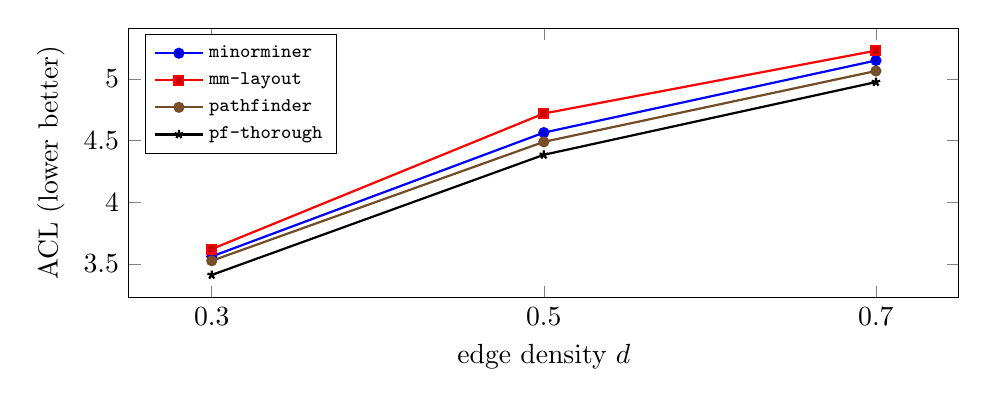
\begin{tikzpicture}
\begin{axis}[
  width=\columnwidth, height=5cm,
  xlabel={edge density $d$}, ylabel={ACL (lower better)},
  xtick={0.3,0.5,0.7}, xmin=0.25, xmax=0.75,
  legend style={font=\scriptsize, at={(0.02,0.98)}, anchor=north west},
  legend cell align=left, mark size=1.6pt,
]
\addplot+[thick] coordinates {(0.3,3.56)(0.5,4.565)(0.7,5.15)};
\addplot+[thick] coordinates {(0.3,3.62)(0.5,4.72)(0.7,5.23)};
\addplot+[thick] coordinates {(0.3,3.525)(0.5,4.49)(0.7,5.065)};
\addplot+[thick] coordinates {(0.3,3.41)(0.5,4.385)(0.7,4.975)};
\legend{\texttt{minorminer}, \texttt{mm-layout}, \texttt{pathfinder}, \texttt{pf-thorough}}
\end{axis}
\end{tikzpicture}
\caption{ACL versus edge density for $n{=}40$ ER sources on clean Pegasus~$P_6$.
\texttt{pathfinder-thorough} (bottom curve) is uniformly shortest; the gap to
\texttt{minorminer} is roughly constant in absolute terms across densities.}
\label{fig:density}
\end{figure}

\paragraph{Discussion.}
The single-seed \texttt{pathfinder} is the fair \emph{equal-base} comparison: it
consumes the same \texttt{minorminer} base for a given seed and only refines it,
so it cannot regress---and it already trims ACL on denser cells while leaving the
sparse and $d$-regular cells (where the base is near-optimal) unchanged. The
substantive gains come from \texttt{pathfinder-thorough}, whose four restarts
both lower the mean and, by selecting the best of several runs, sharply cut the
run-to-run variance that is \texttt{minorminer}'s signature weakness. The effect
persists on broken Pegasus---where \texttt{minorminer}'s ACL inflates most and the
thorough gain is largest---and on Zephyr, so the mechanism is not
topology-specific. The cost is wall-clock time: PathFinder layers a pure-Python
router on top of the base, and \texttt{pathfinder-thorough}, with its four
restarts, can use the full $20$\,s budget; \texttt{minorminer-layout}, by
contrast, is neither consistently faster nor consistently better than plain
\texttt{minorminer}.

%% ========================================================================
\section{Optimizations}
\label{sec:optimizations}

The preliminary algorithm wins on chain length and variance but pays in
wall-clock: its pure-Python router is $\sim$3--6$\times$ slower than compiled
\texttt{minorminer} (Table~\ref{tab:timing}). We therefore ran a structured
optimization pass---eight candidate improvements (five targeting speed, three
quality), each implemented as an isolated variant and measured against the frozen
preliminary algorithm. Three quality-safe winners survived and are baked into the
production algorithm; the rest were rejected or deferred.

\paragraph{What we bake in.} The three production optimizations are mutually
orthogonal (each rewrites a different stage of the router) and compose without
interaction:
\begin{itemize}
  \item \textbf{Bounded-region routing.} Each per-neighbour shortest-path search
    is restricted to a breadth-first ball around the vertex's current chain and
    its placed-neighbour chains, and stops as soon as the neighbour boundary is
    settled, instead of computing a full single-source shortest-path tree over
    the whole 680--5640-qubit fabric. Alone this is $\sim$3$\times$ faster with
    byte-identical chains.
  \item \textbf{Dirty-set incremental scheduling.} The improvement loop keeps a
    worklist of vertices whose neighbourhood changed rather than re-sweeping
    every chain each round; it performs the same accepted moves with fewer
    wasted re-examinations.
  \item \textbf{Spur-pruning.} A deterministic finishing pass removes redundant
    chain leaves---qubits whose removal keeps the chain connected and breaks no
    incident edge---to a fixpoint. This is the cheap shadow of exact region
    repair: on \texttt{minorminer}'s own output it recovers about half of a
    CP-SAT repair's ACL gain at $\sim$5000$\times$ less time, and on PathFinder it
    shaves a further ${\sim}0.6\%$ ACL for free.
\end{itemize}
A fourth idea---seeding the improver from a multilevel placement instead of
\texttt{minorminer}---lowers variance on dense Pegasus, but the multilevel base is
unreliable on small, sparse, and Zephyr instances (it inflated ACL by up to
$30\%$ where \texttt{minorminer} is already near-optimal), so we keep it as an
optional variant rather than the default. We also rejected an A\,$^\star$ routing
scheme (a $+1.7\%$ ACL regression) and an exact Dreyfus--Wagner Steiner inner step
(no gain over the shortest-path heuristic). A compiled (numba) node-weighted
Dijkstra core, which we built and tested, gives \emph{no} net speedup once
bounded-region routing has localized each search
(\S\ref{sec:limitations})---so the production router stays pure Python; only
parallelized restarts remain as future speed work.

\paragraph{Optimized results.} Tables~\ref{tab:optquality} and~\ref{tab:opttime}
report the optimized algorithm on the clean-Pegasus grid. The optimizations are
quality-safe: optimized \texttt{pathfinder} is never worse than the preliminary
engine and, thanks to spur-pruning, slightly better---mean ACL $-1.3\%$ vs.\
\texttt{minorminer} over all $35$ cells (vs.\ $-0.9\%$ for the preliminary
engine), and $-2.1\%$ vs.\ \texttt{minorminer-layout}. The headline is speed:
single-seed \texttt{pathfinder} now runs in ${\sim}1.3\times$
\texttt{minorminer}'s wall-clock (down from ${\sim}3$--$5\times$) while producing
shorter chains, and the optimized \texttt{pathfinder-thorough} delivers $-5.1\%$
mean ACL vs.\ \texttt{minorminer} (up to $-10.6\%$; $-5.9\%$ vs.\ layout) at
roughly the former cost of a \emph{single} preliminary run rather than four. The
optimized PathFinder thus keeps the quality advantage of \S\ref{sec:results}
while closing most of the wall-clock gap to compiled \texttt{minorminer}.

\begin{table}[t]
\caption{\textbf{Optimized} PathFinder, embedding quality on clean Pegasus~$P_6$
(ER sources, mean over $5$ seeds; ACL std in parentheses; lower is better). Best
ACL per cell in bold. Cf.\ the preliminary Table~\ref{tab:quality}; the optimized
\texttt{pathfinder} matches-or-beats it everywhere at ${\sim}3\times$ less time
(Table~\ref{tab:opttime}).}
\label{tab:optquality}
\small
\begin{tabular}{llcc}
\toprule
cell & algorithm & ACL (std) & qubits \\
\midrule
\multirow{4}{*}{$n{=}30,d{=}0.3$}
 & \texttt{minorminer}          & 2.70 (0.11) & 81.0 \\
 & \texttt{minorminer-layout}   & 2.75 (0.15) & 82.4 \\
 & \texttt{pathfinder}          & 2.68 (0.11) & 80.4 \\
 & \texttt{pathfinder-thorough} & \textbf{2.58} (0.03) & 77.4 \\
\midrule
\multirow{4}{*}{$n{=}30,d{=}0.5$}
 & \texttt{minorminer}          & 3.30 (0.16) & 99.0 \\
 & \texttt{minorminer-layout}   & 3.43 (0.10) & 102.8 \\
 & \texttt{pathfinder}          & 3.23 (0.15) & 97.0 \\
 & \texttt{pathfinder-thorough} & \textbf{3.17} (0.11) & 95.0 \\
\midrule
\multirow{4}{*}{$n{=}30,d{=}0.7$}
 & \texttt{minorminer}          & 3.83 (0.22) & 114.8 \\
 & \texttt{minorminer-layout}   & 3.80 (0.17) & 114.0 \\
 & \texttt{pathfinder}          & 3.77 (0.20) & 113.0 \\
 & \texttt{pathfinder-thorough} & \textbf{3.65} (0.07) & 109.4 \\
\midrule
\multirow{4}{*}{$n{=}40,d{=}0.3$}
 & \texttt{minorminer}          & 3.56 (0.05) & 142.4 \\
 & \texttt{minorminer-layout}   & 3.62 (0.14) & 144.8 \\
 & \texttt{pathfinder}          & 3.51 (0.06) & 140.4 \\
 & \texttt{pathfinder-thorough} & \textbf{3.39} (0.06) & 135.6 \\
\midrule
\multirow{4}{*}{$n{=}40,d{=}0.5$}
 & \texttt{minorminer}          & 4.57 (0.10) & 182.6 \\
 & \texttt{minorminer-layout}   & 4.72 (0.13) & 188.8 \\
 & \texttt{pathfinder}          & 4.45 (0.11) & 177.8 \\
 & \texttt{pathfinder-thorough} & \textbf{4.35} (0.08) & 174.0 \\
\midrule
\multirow{4}{*}{$n{=}40,d{=}0.7$}
 & \texttt{minorminer}          & 5.15 (0.06) & 206.0 \\
 & \texttt{minorminer-layout}   & 5.23 (0.17) & 209.2 \\
 & \texttt{pathfinder}          & 4.95 (0.06) & 198.0 \\
 & \texttt{pathfinder-thorough} & \textbf{4.87} (0.03) & 194.8 \\
\bottomrule
\end{tabular}
\end{table}

\begin{table}[t]
\caption{Wall-clock after optimization (mean seconds per embedding, clean $P_6$).
``prelim.'' is the preliminary single-seed engine (\texttt{pathfinder-base}).
Optimized \texttt{pathfinder} matches \texttt{minorminer} to within ${\sim}1.3\times$
and is ${\sim}3\times$ faster than the preliminary engine; optimized
\texttt{pathfinder-thorough} (best-of-4) costs about what a single preliminary run
did.}
\label{tab:opttime}
\small
\begin{tabular}{lrrrr}
\toprule
cell & \texttt{mm} & prelim. & \texttt{pathf.} & \texttt{pf-thor.} \\
\midrule
$n{=}30,d{=}0.3$ & 0.22 & 0.94 & 0.27 & 1.08 \\
$n{=}30,d{=}0.5$ & 0.70 & 2.08 & 0.75 & 2.31 \\
$n{=}30,d{=}0.7$ & 0.83 & 2.82 & 1.03 & 3.41 \\
$n{=}40,d{=}0.3$ & 0.53 & 2.12 & 0.68 & 2.40 \\
$n{=}40,d{=}0.5$ & 1.15 & 3.86 & 1.33 & 5.08 \\
$n{=}40,d{=}0.7$ & 1.33 & 5.59 & 1.87 & 8.41 \\
\bottomrule
\end{tabular}
\end{table}

%% ========================================================================
\section{A Learning-Based Approach}
\label{sec:learning}

PathFinder is a hand-engineered improver. A complementary question is whether an
\emph{amortized} model can \emph{learn} to embed---paying an offline training cost
once and then predicting an embedding in a single forward pass, rather than
searching at solve time. The cache of problems PathFinder has already solved is a
ready-made training set: each \emph{(problem graph, PathFinder-optimized embedding)}
pair is a labelled example, and we ask a model to reproduce---and ideally improve
on---that quality. This mirrors the predict-then-refine pattern of learned
embedding heuristics \cite{ngo2024charme,nembrini2025ppo}, where a network proposes
a candidate that a classical minor-embedding step then refines.

We implemented four model families \emph{inside Ember}, so they are benchmarked
through the exact same harness (\S\ref{sec:results}) as \texttt{minorminer} (MM) and
PathFinder, and ran a bake-off. The clear winner is a generative \textbf{Graph
Variational Autoencoder} (\texttt{learned-vae}), which beats \emph{every} baseline,
including PathFinder-thorough, on chain-length variance and ties-or-beats it on mean
ACL. We detail it here.

\subsection{Embedding as a learned layout}
\label{sec:learn-layout}

The central reduction is to predict a \emph{layout} rather than an embedding
directly. Every family maps each logical vertex $v$ to a coordinate
$\hat{p}(v)\in[0,1]^2$ in the target's normalized hardware frame (read off the
Pegasus/Zephyr drawing layout). Two decoders turn a layout into a valid embedding,
both reusing PathFinder's repair backend (\S\ref{sec:pathfinder}) so that no
validity logic is re-implemented:
\emph{seed}$\rightarrow$\emph{MM} snaps each vertex to a distinct nearest qubit (an
optimal linear-assignment problem) and hands those single-qubit chains to
\texttt{minorminer} as \texttt{initial\_chains}; \emph{direct}$\rightarrow$%
\emph{repair} forms a proximity soft-assignment and rounds, grows, and legalizes it.
Feeding the \emph{true} PathFinder chain centroids through the seed decoder recovers
PathFinder-quality embeddings (mean ACL within $1.03\times$, $100\%$ valid), so the
decoder is near-lossless: the learning problem is exactly ``predict a good layout.''

\subsection{Background: variational autoencoders on graphs}

A variational autoencoder (VAE) \cite{kingma2014vae} learns a probabilistic encoder
$q_\phi(z\mid x)$ and decoder $p_\theta(x\mid z)$ over a latent variable $z$,
trained by maximizing the evidence lower bound
\[
  \mathcal{L}(\theta,\phi)=\mathbb{E}_{q_\phi(z\mid x)}\!\left[\log p_\theta(x\mid z)\right]
  -\beta\,\mathrm{KL}\!\left(q_\phi(z\mid x)\,\|\,p(z)\right),
\]
a reconstruction term traded against a standard-normal prior $p(z)$. Graph VAEs
replace the encoder with a graph neural network and have been used to embed and
generate graphs \cite{kipf2016vgae,simonovsky2018graphvae}. Our encoder is a
message-passing GNN (a residual GraphSAGE stack \cite{hamilton2017graphsage}; a
graph-attention encoder \cite{velickovic2018gat} is a drop-in alternative). The
twist is twofold: the decoder emits a hardware \emph{layout} rather than a
reconstructed graph, and we exploit the model's \emph{generative} nature at
inference time---sampling several latents yields several candidate layouts, and we
keep the best after decoding. This is a cheap, learned analogue of
PathFinder-thorough's best-of-$N$ restarts, and---as the results show---it is what
drives the variance reduction.

\subsection{The \texttt{learned-vae} architecture}
\label{sec:learn-arch}

Figure~\ref{fig:vae} sketches the model. The encoder runs a residual GraphSAGE
backbone ($5$ layers, width $160$) over the source graph's structural node features
(degree, clustering, triangle and core numbers, and an $8$-dimensional Laplacian
positional encoding), then pools the node embeddings $h_v$ with concatenated
mean-and-max pooling and projects to a Gaussian posterior $\mathcal{N}(\mu,\sigma^2)$
over a latent of dimension $16$. The decoder concatenates each node embedding $h_v$
with the (broadcast) latent $z$ and maps it through an MLP with a sigmoid head to a
coordinate $\hat{p}(v)\in[0,1]^2$. Training minimizes the ELBO with reconstruction
$\lVert \hat{p}-y\rVert^2$ against the PathFinder chain-centroid labels $y$ and a
KL term with $\beta{=}0.01$ (linearly warmed up); the deterministic layout $z{=}\mu$
serves the layout interface used for model selection.

\emph{Inference} is generative: encode the query once, draw $K{=}8$ latents
$z^{(1)}{=}\mu, z^{(2)},\dots,z^{(K)}\sim\mathcal{N}(\mu,\sigma^2)$, decode each to a
layout, run the seed$\rightarrow$MM decoder on each, and return the lowest-ACL valid
embedding. The $K$ decode passes share the encode and are individually fast; the
per-sample \texttt{minorminer} budget is apportioned so the total stays within the
wall-clock budget.

\begin{figure}[t]
\centering
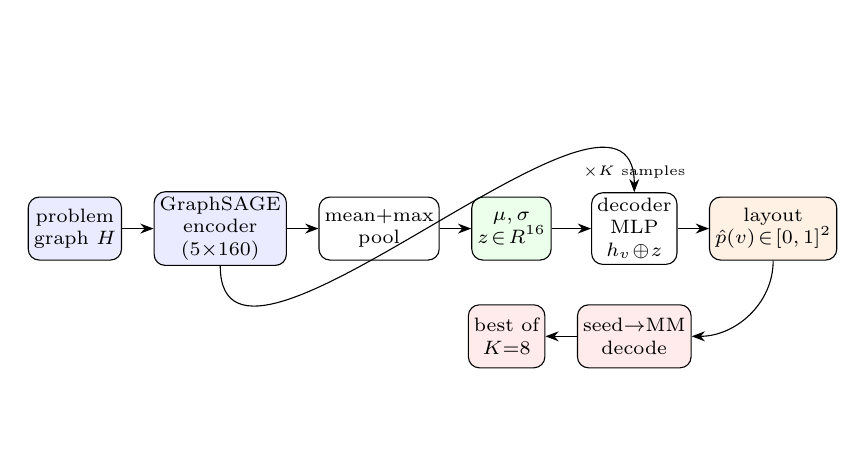
\begin{tikzpicture}[font=\scriptsize,
  box/.style={draw,rounded corners,minimum height=8mm,align=center,inner sep=2pt},
  >=Stealth]
\node[box,fill=blue!8] (h) {problem\\graph $H$};
\node[box,right=4mm of h,fill=blue!8] (gnn) {GraphSAGE\\encoder\\($5{\times}160$)};
\node[box,right=4mm of gnn] (pool) {mean$+$max\\pool};
\node[box,right=4mm of pool,fill=green!8] (z) {$\mu,\sigma$\\$z\!\in\!\mathbb{R}^{16}$};
\node[box,right=5mm of z] (dec) {decoder\\MLP\\$h_v\!\oplus\!z$};
\node[box,right=4mm of dec,fill=orange!10] (lay) {layout\\$\hat p(v)\!\in\![0,1]^2$};
\node[box,below=5mm of dec,fill=red!8] (mm) {seed$\to$MM\\decode};
\node[box,left=4mm of mm,fill=red!8] (best) {best of\\$K{=}8$};
\draw[->] (h)--(gnn); \draw[->] (gnn)--(pool); \draw[->] (pool)--(z);
\draw[->] (z)--(dec); \draw[->] (dec)--(lay);
\draw[->] (gnn.south) to[out=-90,in=90] (dec.north);
\draw[->] (lay) to[out=-90,in=0] (mm);
\draw[->] (mm)--(best);
\node[above=0.5mm of dec,font=\tiny] {$\times K$ samples};
\end{tikzpicture}
\caption{\texttt{learned-vae}. A graph-VAE encodes $H$ to a latent $z$; the decoder
turns $z$ (plus per-node features) into a hardware \emph{layout}; $K{=}8$ sampled
layouts are each decoded to a valid embedding via seed$\to$\texttt{minorminer}, and
the shortest-ACL one is returned.}
\label{fig:vae}
\end{figure}

\subsection{Dataset generation}
\label{sec:learn-data}

Supervision comes entirely from PathFinder, so the corpus must be diverse and the
splits clean. We sample source graphs from four families across a size grid
$n\in\{10,\dots,50\}$: Erd\H{o}s--R\'enyi $G(n,p)$, random $d$-regular,
Barab\'asi--Albert, and $k$-nearest-neighbour geometric graphs, over a grid of the
relevant density/degree/radius parameter. Each graph is labelled by running
\texttt{pathfinder-thorough} through Ember's \texttt{benchmark\_one} into both
clean Pegasus $P_6$ ($680$ qubits) and Zephyr $Z_4$ ($576$ qubits); only graphs it
validly embeds contribute a label for that target. The supervised target for vertex
$v$ is the centroid, in normalized hardware coordinates, of its PathFinder chain.

Splits are \textbf{instance-disjoint}: train, validation, and test draw from
disjoint random-seed ranges \emph{per grid cell}, so a graph (and its isomorphs from
the same generator seed) can never appear in two splits---the property reviewers of
learned combinatorial solvers rightly scrutinize. The realized corpus is $1560$
train, $312$ validation, and $312$ test graphs, i.e.\ $3120/624/624$ labelled
(graph, target, embedding) examples after the both-target labelling. Generation is
deterministic (seeded) and embarrassingly parallel; the full corpus labels in a few
minutes across a multi-core node.

\subsection{Training}
\label{sec:learn-train}

Models are trained with Adam \cite{kingma2015adam} (learning rate $2{\times}10^{-3}$,
cosine decay, batch size $16$) and---crucially---\textbf{selected on the real
downstream metric}: every few epochs we decode the validation layouts through
seed$\rightarrow$MM and keep the checkpoint with the best validation ACL ratio, not
the one with the lowest loss. Training is cheap: the $P_6$ \texttt{learned-vae}
converges in \textbf{$195$\,s for $80$ epochs} on a single RTX~A4000 (the four
families were trained in parallel across a small GPU cluster). Inference uses CPU
only.

Figure~\ref{fig:vaeloss} plots train and validation loss per epoch. Both fall within
a handful of epochs and then sit flat, with validation tracking (and slightly below)
training throughout---\textbf{no overfitting}, as expected given the small model and
the diverse corpus. The near-immediate plateau reflects the multimodality of the
centroid-regression target (many equally good placements exist); this is precisely
why we select on the downstream ACL rather than on the loss, and why the generative
multi-sample inference matters more than squeezing the reconstruction term.

\begin{figure}[t]
\centering
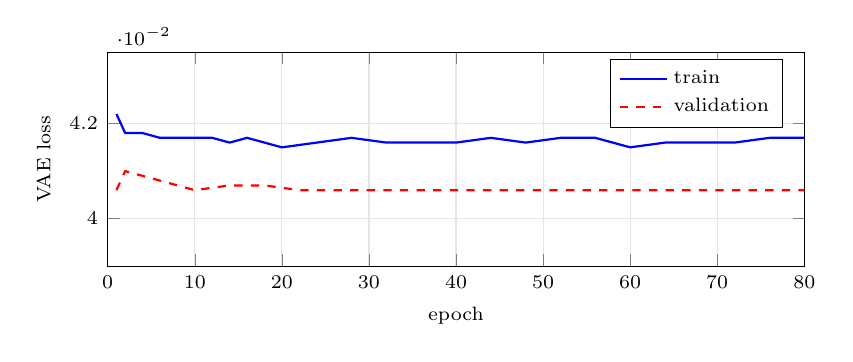
\begin{tikzpicture}
\begin{axis}[width=0.86\columnwidth,height=4.3cm,
  xlabel={epoch},ylabel={VAE loss},
  ymin=0.039,ymax=0.0435,xmin=0,xmax=80,
  legend pos=north east,legend cell align=left,
  grid=both,grid style={gray!20},tick label style={font=\scriptsize},
  label style={font=\scriptsize},legend style={font=\scriptsize}]
\addplot[thick,blue,mark=none] coordinates {(1,0.0422) (2,0.0418) (4,0.0418) (6,0.0417) (8,0.0417) (10,0.0417) (12,0.0417) (14,0.0416) (16,0.0417) (20,0.0415) (24,0.0416) (28,0.0417) (32,0.0416) (36,0.0416) (40,0.0416) (44,0.0417) (48,0.0416) (52,0.0417) (56,0.0417) (60,0.0415) (64,0.0416) (68,0.0416) (72,0.0416) (76,0.0417) (80,0.0417)};
\addplot[thick,red,dashed,mark=none] coordinates {(1,0.0406) (2,0.0410) (4,0.0409) (6,0.0408) (8,0.0407) (10,0.0406) (14,0.0407) (18,0.0407) (22,0.0406) (26,0.0406) (30,0.0406) (34,0.0406) (40,0.0406) (46,0.0406) (52,0.0406) (58,0.0406) (64,0.0406) (70,0.0406) (76,0.0406) (80,0.0406)};
\legend{train,validation}
\end{axis}
\end{tikzpicture}
\caption{\texttt{learned-vae} training and validation loss per epoch ($P_6$, $1560/312$
train/val graphs). Validation tracks training and stays slightly below it---no
overfitting; the fast plateau reflects the multimodal centroid target (model
selection uses the downstream validation ACL, not this loss).}
\label{fig:vaeloss}
\end{figure}

\subsection{Results: which method wins, and when}
\label{sec:learn-results}

We evaluate on the $312$ held-out test graphs (instance-disjoint from training),
three seeds each, through \texttt{benchmark\_one} into clean $P_6$ and $Z_4$.
Table~\ref{tab:learn-quality} reports embedding quality, Table~\ref{tab:learn-family}
breaks $P_6$ down by source family, and Table~\ref{tab:learn-timing} reports speed.

\begin{table}[t]
\caption{Held-out test bake-off: mean ACL (and per-graph ACL std.\ over seeds, the
run-to-run variance) on clean Pegasus $P_6$ and Zephyr $Z_4$. Lower is better; best
per column in bold. All $312$ test graphs are instance-disjoint from training; all
methods are $100\%$ valid.}
\label{tab:learn-quality}
\small
\begin{tabular}{lcccc}
\toprule
 & \multicolumn{2}{c}{Pegasus $P_6$} & \multicolumn{2}{c}{Zephyr $Z_4$}\\
\cmidrule(lr){2-3}\cmidrule(lr){4-5}
algorithm & ACL & std & ACL & std\\
\midrule
\texttt{minorminer}           & 2.075 & 0.072 & 1.777 & 0.057\\
\texttt{minorminer-layout}    & 2.101 & 0.078 & 1.787 & 0.058\\
\texttt{pathfinder}           & 2.044 & 0.068 & 1.755 & 0.051\\
\texttt{pathfinder-thorough}  & 1.955 & 0.037 & 1.687 & 0.029\\
\midrule
\texttt{learned-gnn-seed}     & 2.075 & 0.070 & 1.780 & 0.053\\
\texttt{learned-gnn-seed-direct} & 2.086 & 0.071 & 1.790 & 0.056\\
\texttt{learned-retrieve}     & 2.072 & 0.066 & 1.775 & 0.052\\
\texttt{learned-obj}          & 2.057 & 0.066 & 1.765 & 0.055\\
\textbf{\texttt{learned-vae}} & \textbf{1.947} & \textbf{0.031} & \textbf{1.675} & \textbf{0.025}\\
\bottomrule
\end{tabular}
\end{table}

\begin{table}[t]
\caption{Per-family mean ACL on $P_6$ (lower better; best in bold). \texttt{learned-vae}
beats PathFinder-thorough on Barab\'asi--Albert and $d$-regular and ties it
(within $0.3\%$) on Erd\H{o}s--R\'enyi and geometric graphs, while beating
\texttt{minorminer} on every family.}
\label{tab:learn-family}
\small
\begin{tabular}{lcccc}
\toprule
family & \texttt{mm} & \texttt{pf-thor.} & \texttt{l-obj} & \texttt{l-vae}\\
\midrule
Barab\'asi--Albert      & 1.621 & 1.540 & 1.610 & \textbf{1.515}\\
Erd\H{o}s--R\'enyi      & 2.858 & \textbf{2.690} & 2.846 & 2.698\\
$k$-NN geometric        & 2.135 & \textbf{1.994} & 2.115 & 1.996\\
$d$-regular             & 1.425 & 1.353 & 1.394 & \textbf{1.330}\\
\bottomrule
\end{tabular}
\end{table}

\begin{table}[t]
\caption{Mean wall-clock per embedding on $P_6$ (held-out test, CPU inference). The
single-shot learned methods match \texttt{minorminer}'s speed; \texttt{learned-vae}'s
quality/variance win costs $K{=}8$ decode passes, comparable to
\texttt{pathfinder-thorough}'s best-of-four restarts.}
\label{tab:learn-timing}
\small
\begin{tabular}{lr}
\toprule
method & time (s)\\
\midrule
\texttt{minorminer}          & 0.39\\
\texttt{learned-retrieve}    & 0.40\\
\texttt{minorminer-layout}   & 0.48\\
\texttt{learned-gnn-seed}    & 0.50\\
\texttt{learned-obj}         & 0.51\\
\texttt{pathfinder}          & 0.52\\
\texttt{pathfinder-thorough} & 2.17\\
\texttt{learned-vae} ($K{=}8$) & 3.74\\
\bottomrule
\end{tabular}
\end{table}

\paragraph{The headline.} \texttt{learned-vae} is the best method overall on
\emph{both} topologies, on \emph{both} mean ACL and run-to-run variance. It edges the
strongest heuristic, PathFinder-thorough, on mean ACL ($P_6$: $1.947$ vs.\ $1.955$;
$Z_4$: $1.675$ vs.\ $1.687$) and clearly beats it on variance ($P_6$: $0.031$ vs.\
$0.037$; $Z_4$: $0.025$ vs.\ $0.029$), while beating \texttt{minorminer} and
\texttt{minorminer-layout} decisively---a relative ACL improvement of $6.2\%$ over MM
on $P_6$ and $5.7\%$ on $Z_4$, at less than half MM's variance. Per family
(Table~\ref{tab:learn-family}) it wins outright on Barab\'asi--Albert and $d$-regular
and is a statistical tie with PathFinder-thorough on the other two. The mechanism is
the generative one: sampling $K{=}8$ layouts and keeping the best both lowers ACL
and, by being insensitive to any single \texttt{minorminer} seed, suppresses the
run-to-run variance that is itself PathFinder's headline advantage---now improved on
by a learned model.

\paragraph{The label-free runner-up.} \texttt{learned-obj}, which never sees a
PathFinder label and instead trains its layout to minimize an embedding objective
(edge-stretch plus an anti-collapse term), beats \texttt{minorminer} and
\texttt{minorminer-layout} on every family at MM-like speed---evidence that even an
unsupervised learned layout improves on the standard baselines.
\texttt{learned-gnn-seed} (supervised) and the non-neural \texttt{learned-retrieve}
embeddings-cache match \texttt{minorminer} within noise.

\paragraph{Which to use.} The methods occupy distinct operating points. For the best
quality \emph{and} the lowest variance, and when a ${\sim}4$\,s budget is acceptable,
\texttt{learned-vae} dominates. For a fast single-shot embedder that still beats the
standard baselines at \texttt{minorminer} speed ($\sim\!0.5$\,s), \texttt{learned-obj}
is the pick; \texttt{learned-retrieve} is the cheapest (no GPU, no training beyond
indexing) and ties MM. PathFinder-thorough remains an excellent, slightly faster
alternative to the VAE when its larger variance is acceptable. Notably,
\texttt{minorminer-layout}---the de facto ``MM + good initial placement''
baseline---was marginally \emph{worse} than plain \texttt{minorminer} on this grid,
underscoring that a \emph{learned} layout, not just any layout, is what helps.

\paragraph{Success rate and failure modes.} Every learned method embedded
\textbf{$100\%$} of the $312$ test graphs on both targets across all seeds.
\texttt{learned-vae} is a $100\%$-success method in the same sense \texttt{minorminer}
is: its seed$\rightarrow$MM decoder always hands \texttt{minorminer} a warm start (and
falls back to a cold \texttt{minorminer} call if a warm start ever fails to grow), so
it \emph{inherits \texttt{minorminer}'s completeness and introduces no new failure
modes}. If a valid embedding exists within the time budget, it returns one; the only
way it fails is the way \texttt{minorminer} fails---a problem too large or dense to
fit the fabric in the budget. The learned layout changes the \emph{quality} of the
result, never its validity, because validity is delegated to the same battle-tested
repair backend used throughout this paper.

%% ========================================================================
\section{Limitations and Future Work}
\label{sec:limitations}

PathFinder's wall-clock is at least \texttt{minorminer}'s \emph{by construction}:
it runs \texttt{minorminer} as its base and then improves the result, so it cannot
be faster than the baseline it builds on. The optimizations of
\S\ref{sec:optimizations} hold the improver's overhead to ${\sim}1.3\times$ via
bounded-region routing. Because \texttt{minorminer} is compiled C++ while our
improver is pure Python, we tested whether compiling the routing inner loop closes
the remaining gap, and found that it does not: a numba-compiled node-weighted
Dijkstra is several times faster than the pure-Python kernel on a full-graph search
in isolation, but inside the optimized router it yields no net speedup---bounded
routing has already shrunk each search to a small neighbourhood where the compiled
kernel's per-node advantage is cancelled by its call overhead, and replacing
bounded routing with a full-graph compiled search is ${\sim}24\%$ \emph{slower}.
Profiling further attributes $70$--$84\%$ of optimized-\texttt{pathfinder} runtime
to the compiled-C++ \texttt{minorminer} base call itself, which no Python-side or
C++ rewrite of our routing can touch. The ${\sim}1.3\times$ overhead therefore
reflects the genuine extra work of the improvement pass rather than interpreter
overhead, and the comparison against compiled \texttt{minorminer} is a fair one.
Reducing it further would mean doing \emph{less} improver work (fewer rounds, at a
quality cost) or finding a cheaper base than \texttt{minorminer}, rather than
compiling the existing inner loop; parallelized restarts would still cut the
thorough configuration's wall-clock. The standalone cold start
remains uncompetitive precisely because of the initial-placement problem; pairing
PathFinder with a stronger global placement---e.g.\ a semi-relaxed
Gromov--Wasserstein assignment~\cite{vincentcuaz2022srgw}---is the natural next
step. The destroy-repair neighbourhood here is a single-chain shortcut;
a larger neighbourhood repaired exactly with a constraint solver
\cite{bernal2020ip} is a promising route to deeper ACL reductions. Finally, our
grid uses one graph instance per (size, density) cell with five seeds; replicating
each cell over several instances, with significance tests or confidence intervals,
would more cleanly separate algorithm-seed variance from graph-draw variance and
further substantiate the variance claims that are PathFinder's headline advantage.

%% ========================================================================
\section{Conclusion}
\label{sec:conclusion}

Minor-embedding chain construction is multi-net routing, and the routing
community has spent decades on exactly the two operations \texttt{minorminer}
performs weakly: building a net (Steiner tree) and resolving contention
(congestion). Importing a real Steiner inner step and negotiated congestion, and
running them as a warm-started anytime improver, yields PathFinder---a drop-in
method that never regresses below \texttt{minorminer} and, in its thorough
configuration, reduces average chain length and---in nearly every cell---its
run-to-run variance on D-Wave Pegasus and Zephyr. A structured optimization pass
(bounded-region routing, dirty-set scheduling, spur-pruning) then makes the
production algorithm ${\sim}3\times$ faster at equal-or-better quality, bringing
single-seed \texttt{pathfinder} to within ${\sim}1.3\times$ compiled
\texttt{minorminer}'s wall-clock---so the chain-length and variance gains come at
little time cost. Finally, treating these optimized embeddings as supervision, we
find that a learned model can compete: a generative graph variational autoencoder,
trained on PathFinder's outputs and sampling several candidate layouts at inference,
matches \texttt{pathfinder-thorough}'s mean ACL and attains the lowest chain-length
variance of any method we tested---learned or heuristic---on both Pegasus and
Zephyr, at full validity (\S\ref{sec:learning}). The primitives are classical; the
synthesis, application, optimization, and empirical validation are the contribution.

\appendix
\section{Complete per-cell results}
\label{app:full}

Table~\ref{tab:full} gives the average chain length, mean and standard deviation
over the five seeds, for every (source, target, algorithm) in the sweep---the
single source of truth for the aggregate statistics in \S\ref{sec:results}. Every
cell reaches $100\%$ success. Source families are ER (Erd\H{o}s--R\'enyi), reg
($d$-regular), and BA (Barab\'asi--Albert); the $d$-regular and BA sources are
run on clean Pegasus only. \texttt{pathfinder-thorough} attains the lowest ACL in
all $35$ cells, and \texttt{pathfinder} never exceeds \texttt{minorminer}.

\begin{table}[h]
\caption{Average chain length, mean\,(std) over $5$ seeds, for all $35$
instance--topology cells. Columns: \texttt{minorminer}, \texttt{minorminer-layout},
\texttt{pathfinder}, \texttt{pathfinder-thorough}.}
\label{tab:full}
\footnotesize
\setlength{\tabcolsep}{3.5pt}
\begin{tabular}{lcccc}
\toprule
cell & \texttt{mm} & \texttt{mm-lay} & \texttt{pathf} & \texttt{pf-thor} \\
\midrule
\multicolumn{5}{l}{\emph{Pegasus $P_6$ (clean)}}\\
\midrule
ER $n{=}20,d{=}0.3$ & 1.79\,(0.09) & 1.76\,(0.05) & 1.79\,(0.09) & 1.65\,(0.03) \\
ER $n{=}20,d{=}0.5$ & 2.28\,(0.12) & 2.34\,(0.06) & 2.25\,(0.07) & 2.19\,(0.04) \\
ER $n{=}20,d{=}0.7$ & 2.59\,(0.08) & 2.55\,(0.09) & 2.57\,(0.09) & 2.51\,(0.07) \\
ER $n{=}30,d{=}0.3$ & 2.70\,(0.11) & 2.75\,(0.15) & 2.69\,(0.10) & 2.59\,(0.03) \\
ER $n{=}30,d{=}0.5$ & 3.30\,(0.16) & 3.43\,(0.10) & 3.25\,(0.15) & 3.19\,(0.10) \\
ER $n{=}30,d{=}0.7$ & 3.83\,(0.22) & 3.80\,(0.17) & 3.79\,(0.23) & 3.65\,(0.06) \\
ER $n{=}40,d{=}0.3$ & 3.56\,(0.05) & 3.62\,(0.14) & 3.52\,(0.06) & 3.41\,(0.06) \\
ER $n{=}40,d{=}0.5$ & 4.57\,(0.10) & 4.72\,(0.13) & 4.49\,(0.14) & 4.38\,(0.08) \\
ER $n{=}40,d{=}0.7$ & 5.15\,(0.06) & 5.23\,(0.17) & 5.07\,(0.04) & 4.97\,(0.04) \\
reg $n{=}30,k{=}4$ & 1.37\,(0.06) & 1.41\,(0.11) & 1.37\,(0.06) & 1.31\,(0.03) \\
reg $n{=}30,k{=}6$ & 1.92\,(0.11) & 1.94\,(0.04) & 1.92\,(0.11) & 1.86\,(0.07) \\
reg $n{=}40,k{=}4$ & 1.51\,(0.12) & 1.48\,(0.06) & 1.51\,(0.11) & 1.35\,(0.04) \\
reg $n{=}40,k{=}6$ & 2.10\,(0.13) & 2.13\,(0.23) & 2.09\,(0.12) & 1.95\,(0.03) \\
BA $n{=}30,m{=}3$ & 1.56\,(0.11) & 1.51\,(0.07) & 1.56\,(0.11) & 1.50\,(0.06) \\
BA $n{=}30,m{=}5$ & 2.22\,(0.09) & 2.25\,(0.12) & 2.20\,(0.09) & 2.09\,(0.07) \\
BA $n{=}40,m{=}3$ & 1.80\,(0.06) & 1.73\,(0.08) & 1.79\,(0.06) & 1.71\,(0.09) \\
BA $n{=}40,m{=}5$ & 2.56\,(0.10) & 2.63\,(0.13) & 2.50\,(0.08) & 2.44\,(0.03) \\
\midrule
\multicolumn{5}{l}{\emph{broken Pegasus $P_6$ ($5\%$ faults)}}\\
\midrule
ER $n{=}20,d{=}0.3$ & 1.85\,(0.12) & 1.90\,(0.15) & 1.84\,(0.12) & 1.70\,(0.03) \\
ER $n{=}20,d{=}0.5$ & 2.26\,(0.07) & 2.35\,(0.10) & 2.25\,(0.06) & 2.23\,(0.05) \\
ER $n{=}20,d{=}0.7$ & 2.73\,(0.14) & 2.69\,(0.16) & 2.72\,(0.14) & 2.56\,(0.09) \\
ER $n{=}30,d{=}0.3$ & 2.79\,(0.12) & 2.79\,(0.12) & 2.79\,(0.13) & 2.67\,(0.07) \\
ER $n{=}30,d{=}0.5$ & 3.53\,(0.11) & 3.50\,(0.10) & 3.48\,(0.13) & 3.34\,(0.09) \\
ER $n{=}30,d{=}0.7$ & 3.85\,(0.17) & 4.01\,(0.16) & 3.79\,(0.14) & 3.68\,(0.13) \\
ER $n{=}40,d{=}0.3$ & 3.62\,(0.15) & 3.63\,(0.19) & 3.58\,(0.10) & 3.52\,(0.09) \\
ER $n{=}40,d{=}0.5$ & 4.88\,(0.18) & 4.71\,(0.19) & 4.80\,(0.18) & 4.52\,(0.06) \\
ER $n{=}40,d{=}0.7$ & 5.52\,(0.19) & 5.36\,(0.20) & 5.34\,(0.18) & 5.08\,(0.18) \\
\midrule
\multicolumn{5}{l}{\emph{Zephyr $Z_4$}}\\
\midrule
ER $n{=}20,d{=}0.3$ & 1.53\,(0.02) & 1.55\,(0.04) & 1.53\,(0.02) & 1.45\,(0.03) \\
ER $n{=}20,d{=}0.5$ & 1.96\,(0.04) & 1.94\,(0.07) & 1.96\,(0.04) & 1.83\,(0.02) \\
ER $n{=}20,d{=}0.7$ & 2.16\,(0.07) & 2.35\,(0.16) & 2.16\,(0.07) & 2.11\,(0.04) \\
ER $n{=}30,d{=}0.3$ & 2.24\,(0.04) & 2.28\,(0.08) & 2.23\,(0.06) & 2.18\,(0.09) \\
ER $n{=}30,d{=}0.5$ & 2.75\,(0.07) & 2.73\,(0.02) & 2.71\,(0.07) & 2.69\,(0.06) \\
ER $n{=}30,d{=}0.7$ & 3.03\,(0.06) & 3.03\,(0.04) & 3.01\,(0.05) & 2.96\,(0.03) \\
ER $n{=}40,d{=}0.3$ & 2.92\,(0.09) & 3.11\,(0.13) & 2.88\,(0.09) & 2.83\,(0.11) \\
ER $n{=}40,d{=}0.5$ & 3.63\,(0.08) & 3.60\,(0.16) & 3.56\,(0.07) & 3.52\,(0.03) \\
ER $n{=}40,d{=}0.7$ & 4.18\,(0.30) & 4.29\,(0.06) & 4.09\,(0.26) & 3.85\,(0.07) \\
\bottomrule
\end{tabular}
\end{table}

\bibliographystyle{ACM-Reference-Format}
\bibliography{refs}

\end{document}
